\section{COMPRENSIÓN DE LOS DATOS}
El simulador cuenta con un sistema integrado para el control de los vehículos llamado Traffic Manager, este hace uso de toda la información disponible sobre el mapa y los objetos en él, siendo estos la topología de las calles, distancia a los obstáculos y coordenadas de los demás vehículos, para mediante código configurar si se quiere ceder el control del vehículo al sistema o controlarlo nosotros.

Se implementa un módulo de extracción (figura \ref{extraccion}), que consiste en dejar que el sistema cree un vehículo denominado ``jugador'', que será con el que se trabaja, en alguna posición aleatoria del mapa, dejando que el sistema tome control conduciendo el vehículo mediante caminos arbitrarios durante un tiempo definido por 8000 fotogramas, generando datos en forma de imágenes y sus correspondientes etiquetas

\begin{figure}[H]
	\centering
	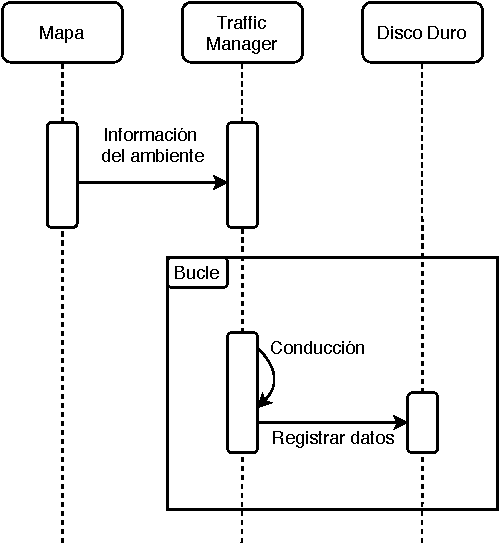
\includegraphics[scale=0.9]{imagenes/arquitectura-extraccion}
	\caption[Diagrama de secuencia de extracción de datos]{Diagrama de secuencia de extracción de datos}
	\label{extraccion}
\end{figure}

estas son de tres tipos

\subsection{ACELERADOR Y DIRECCIÓN}
Es un par de números, el valor del acelerador en un rango $(0, 1)$, indica cuánto por ciento del acelerador está siendo presionado, la dirección es un valor entre $(-1, 1)$, equivalente a dos proporciones en una variable, indicando cuánto se debe girar a la izquierda o a la derecha.

\subsection{PROFUNDIDAD}
CARLA cuenta con una cámara virtual que codifica la profundidad o distancia a objetos en un fotograma, estos valores están codificados como números de 24 bits en una imagen RGB que deben ser normalizados de la siguiente manera:

$$\text{distancia} = \frac{R + G\cdot256 + B\cdot256\cdot256}{256\cdot256\cdot256 - 1} \cdot 1000$$

para obtener las distancias entre 0 y 1000 metros.

\begin{figure}[H]
	\centering
	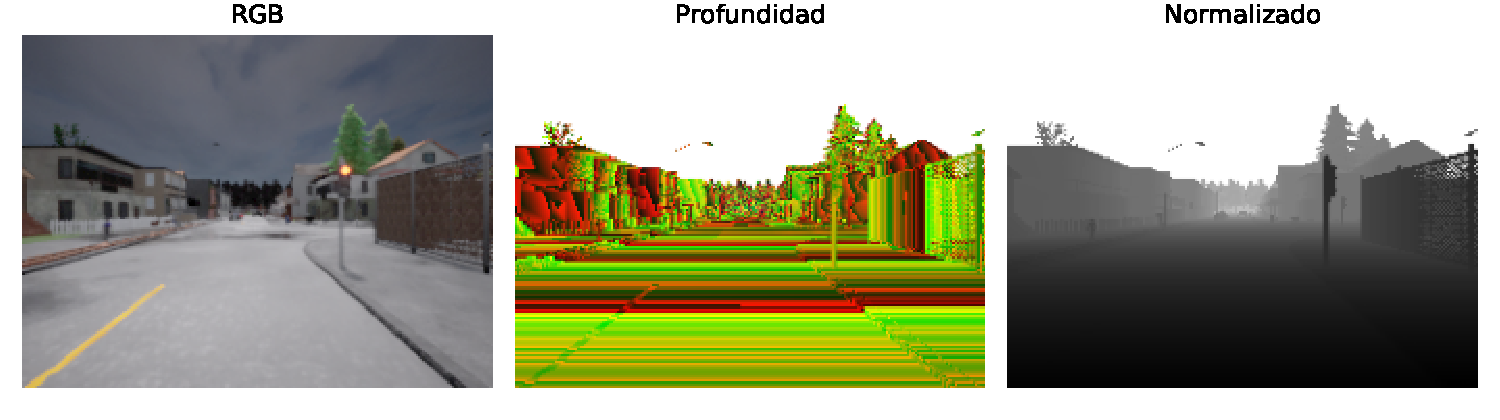
\includegraphics[scale=0.62]{imagenes/depth}
	\caption[Etiquetas de profundidad imagen]{Etiquetas de la profundidad de la imagen}
	\label{depth}
\end{figure}

\subsection{SEGMENTACIÓN SEMÁNTICA}
Igualmente CARLA cuenta con una cámara virtual que permite obtener la segmentación semántica de los objetos en un fotograma, estos datos están codificados como valores de píxeles en el canal rojo, cada valor de la máscara indica a qué clase pertenece el píxel correspondiente a esa coordenada de la imagen.

\begin{center}
	\footnotesize
	\begin{tabular}{|c|c|c|}
		\hline
		Valor mascara & Clase & Código de color\\
		\hline
		$0$ & Nada & \cellcolor{none}\\
		\hline
		$1$ & Edificios & \cellcolor{buildings}\\
		\hline
		$2$ & Cercas & \cellcolor{fences}\\
		\hline
		$3$ & Otro & \cellcolor{other}\\
		\hline
		$4$ & Peatones & \cellcolor{pedestrians}\\
		\hline
		$5$ & Postes & \cellcolor{poles}\\
		\hline
		$6$ & Lineas de carriles & \cellcolor{roadlines}\\
		\hline
		$7$ & Caminos & \cellcolor{roads}\\
		\hline
		$8$ & Aceras & \cellcolor{sidewalks}\\
		\hline
		$9$ & Vegetación & \cellcolor{vegetation}\\
		\hline
		$10$ & Vehículos & \cellcolor{vehicles}\\
		\hline
		$11$ & Paredes & \cellcolor{walls}\\
		\hline
		$12$ & Señales de transito & \cellcolor{trafficsigns}\\
		\hline
	\end{tabular}
	\captionof{table}[Correspondencia numérica de clases de segmentación]{Correspondencia numérica de las clases}\label{clases}
\end{center}

para facilitar la visualización se aplica un código de color descrito por la tabla \ref{clases}, a las clases de píxeles en la imagen.

\begin{figure}[H]
	\centering
	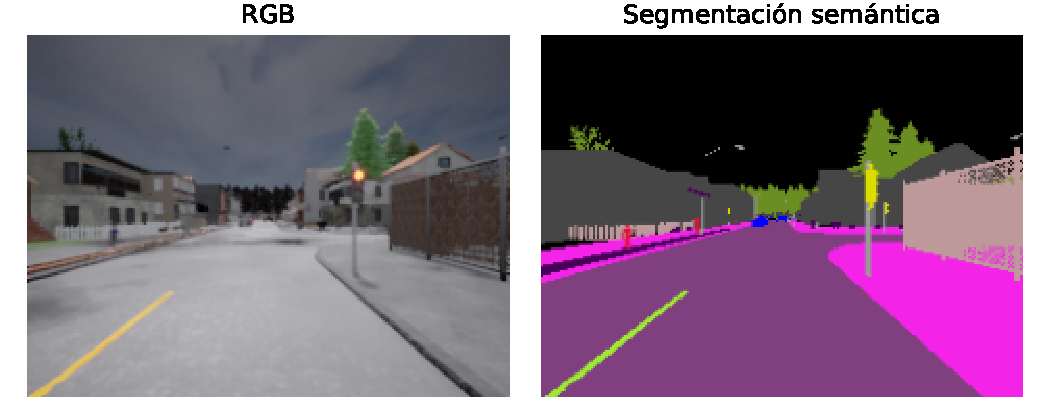
\includegraphics[scale=0.6]{imagenes/semseg}
	\caption[Segmentación semántica con códigos de color]{Segmentación semántica con códigos de color}
	\label{semseg}
\end{figure}

para facilitar el pre procesado de esta información, por cada simulación se genera una carpeta con tres dentro, una para imágenes estándar rgb que es lo que se observa a través de la cámara, una carpeta para las máscaras de la segmentación y una para las profundidades, cada archivo dentro de cada carpeta lleva el mismo nombre. Finalmente para las etiquetas del acelerador y dirección, se crea un archivo CSV que contenga la información de manera tabulada, con cada fila conteniendo las columnas

\begin{itemize}[nosep]
	\item throttle (acelerador): intensidad del acelerador.
	\item brake (freno): intensidad de freno.
	\item steer (aceleración): intensidad de dirección.
	\item junction (intersección): valor booleano sobre si la imagen pertenece o no a una intersección.
\end{itemize}

se tienen múltiples CSVs ya que se crean para cada simulación, y la información se obtiene del estado del vehículo y el mapa.